% !TeX spellcheck = en_GB

\subsection{\acrfull{smote}}
\label{subsection:smote}

	As previously mentioned in \ref{subsection:data-augmentation}, \acrshort{smote} consists of an over-sampling method whose function is to generate synthetic samples in order to populate the minority class in a classification problem by making use of the proper observations that are already contained in the data \cite{Chawla2002}. 
	
	Essentially, this technique works by choosing samples from the less populated class that are represented in the features space, placing a line between two of these samples and then select a point inside the line at a random position. First, an arbitrary sample is picked and then a number of \textit{k} closest neighbours in the feature space are selected from the same class. One of the neighbours are randomly chosen and a synthetic sample is generated \cite{Browniee2020}. The number of neighbours \textit{k} can vary depending on the amount of over-sampling needed. The standard value which is the one proposed in the publication paper is \textit{k = 5} \cite{Chawla2002}. 
	
	For the generation of the synthetic samples, the distance between the feature vector first arbitrarily selected and one of the nearest neighbours is computed. Then, the resulting value is scaled by multiplying it by a random number that lies in the uniform distribution $U(0,1)$. Finally, this new sample, \textit{S}, is added to the initial feature vector and placed in between these two observations in the feature space \cite{Chawla2002}. \textit{S} can be defined as follows:
	\[S = x + u\cdot(x^{R} - x) \]
	where \textit{x} is the arbitrary selected sample the first time, \textit{u} is the random value from $U(0,1)$ and \textit{x\textsuperscript{R}} is one of the closest neighbours \cite{Blagus2013}. In figure \ref{fig:mesh47}, it is shown a graphical representation of the algorithm. In this case, \textit{X} is the original sample for which the closest neighbours are represented as $X_{i}$ where $i=1,2,3,4,5$. The generated samples are $Y_{1}$ and $Y_{2}$ that are placed in the line segments.
	
	\begin{figure}
		\centering
		\captionsetup{justification=centering}
		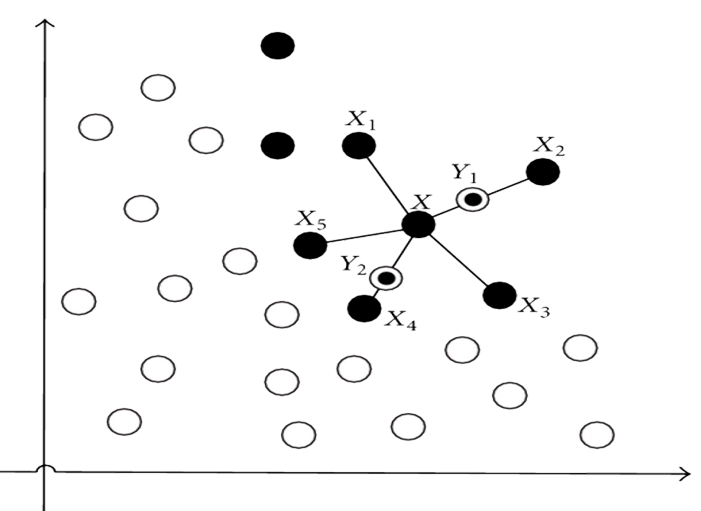
\includegraphics[scale=0.3]{SMOTE}
		\caption{SMOTE algorithm \cite{Xie2015}}
		\label{fig:mesh47}
	\end{figure}

	The common way of applying this technique is in the train set before performing the fit of the model. Usually, an under sampling is performed in the most populated classes and, then, the data augmentation is done for the minority ones \cite{Browniee2020}. Our implementation follows this way of acting and it is explained in section \ref{section:input-data-preparation}.
	
	 